\documentclass[25pt, a0paper, portrait]{tikzposter}

% Encodage et typographie
\usepackage[utf8]{inputenc}
\usepackage[T1]{fontenc}
\usepackage[french,english]{babel}
\usepackage{lmodern}
\usepackage{amsmath, amssymb, amsfonts, dsfont}
\usepackage{graphicx}
\usepackage{tikz}
\usepackage{capt-of}
\usetikzlibrary{shapes,arrows,positioning,fit,backgrounds,calc}
\tikzposterlatexaffectionproofoff
% 1. Définition des couleurs officielles
\definecolor{bleu303}{RGB}{0,62,92}
\definecolor{bleu315}{RGB}{0,104,128}
\definecolor{rouge485}{RGB}{213,43,30}
\definecolor{bleu303pale}{RGB}{204,216,222} 

% 2. Création d'un style de couleur personnalisé
\definecolorstyle{PolyColors}{
    \definecolor{colorOne}{named}{bleu303}
    \definecolor{colorTwo}{named}{bleu315}
    \definecolor{colorThree}{named}{rouge485}
}{
    \colorlet{backgroundcolor}{bleu303pale!30!white}
    \colorlet{framecolor}{bleu303}
    \colorlet{titlebgcolor}{bleu303}
    \colorlet{titlefgcolor}{white}
    \colorlet{blocktitlebgcolor}{bleu303}
    \colorlet{blocktitlefgcolor}{white}
    \colorlet{blockbodybgcolor}{white}
    \colorlet{blockbodyfgcolor}{black}
    \colorlet{innerblocktitlebgcolor}{bleu315}
    \colorlet{innerblocktitlefgcolor}{white}
    \colorlet{innerblockbodybgcolor}{bleu315!10!white}
    \colorlet{innerblockbodyfgcolor}{black}
    \colorlet{notefgcolor}{black}
    \colorlet{notebgcolor}{rouge485!20!white}
    \colorlet{notefrcolor}{rouge485}
}

% 3. Application du thème
\usetheme{Desert}
\usecolorstyle{PolyColors}

\definebackgroundstyle{PolyBackground}{
    \fill[inner sep=0pt, line width=0pt, color=backgroundcolor] (bottomleft) rectangle (topright);
    \node[opacity=0.08] at (current page.center) {
        
\includegraphics[width=1.2\paperwidth]{polytechnique-armes.pdf}
    };
}
\usebackgroundstyle{PolyBackground}

\defineblockstyle{TransparentSlide}{
    titlewidthscale=1, bodywidthscale=1, titleleft,
    titleoffsetx=0pt, titleoffsety=0pt, bodyoffsetx=0pt, bodyoffsety=0pt,
    bodyverticalshift=0pt, roundedcorners=0, linewidth=0pt, titleinnersep=1cm,
    bodyinnersep=1cm
}{
    \ifBlockHasTitle%
        \draw[draw=none, left color=blocktitlebgcolor, right color=blockbodybgcolor, fill opacity=0.85]
           (blocktitle.south west) rectangle (blocktitle.north east);
    \fi%
    \draw[draw=none, fill=blockbodybgcolor, fill opacity=0.85] %
        (blockbody.north west) [rounded corners=30] -- (blockbody.south west) --
        (blockbody.south east) [rounded corners=0]-- (blockbody.north east) -- cycle;
}
\useblockstyle{TransparentSlide}

% 4. Informations du document
\title{\parbox{\linewidth}{\centering \textbf{AudioConditioner}\\[0.3em] \Large Results \& Applications}}
\author{Keyvan Attarian \& Baptiste Arnaudo}
\institute{CSC\_52002\_EP - Multimodal generative AI}

\begin{document}

\maketitle

\begin{columns}

\column{0.5}

\block{\textsc{Application I: Image to Ambient Music}}{
    One direct application of the \textbf{AudioConditioner} framework is generating ambient music and atmospheres based on visual inputs. By passing an image into our pipeline:
    \medskip
    
    \begin{itemize}
        \item We use \textbf{BLIP} to automatically focus on the scene, extracting elements, colors, and objects.
        \item This scene description drives the AudioConditioner pipeline (through the CLAP Descriptor and Stable Audio); we aim to match the mood of the image in the generated audio.
        \item We re-rank the audio candidates using the CLAP cosine similarity filter to prioritize alignment with the initial visual.
    \end{itemize}
    \medskip
    This enables automated soundtrack generation for static artwork, game environments, or visual media.
}

\block{\textsc{Application II: Text Reading with Adaptive Music}}{
    The \textbf{ReadMusic} module combines speech synthesis with adaptive background music scoring to produce narrated audiobooks with adaptive background music.
    \medskip
    
    \begin{center}
    \begin{tikzpicture}[
        node distance=1.5cm and 1.5cm,
        box/.style={rectangle, draw=black, thick, fill=blue!10, text width=6cm, align=center, rounded corners, minimum height=1.5cm},
        arrow/.style={->, thick, >=stealth}
    ]
        \node[box, fill=green!10] (input) {Input Narrative Text};
        \node[box] (chunking) [below=1.5cm of input] {Text Chunking \\ (Max 80 words/chunk)};
        
        \node[box, fill=purple!10] (tts) [below left=2cm and 0.5cm of chunking] {\textbf{F5-TTS Synthesis} \\ Generate Speech \\ resample to 48kHz};
        \node[box, fill=orange!10] (ac) [below right=2cm and 0.5cm of chunking] {\textbf{Audio Conditioner} \\ Generate Music \\ Match Duration};
        
        \node[box] (mixer) [below=10cm of chunking] {Length Matching \\ \& Dual Mixer ($Gains$)};
        \node[box, fill=yellow!10] (fade) [below=1.5cm of mixer] {Cross-fade Appending};
        \node[box, fill=green!10] (output) [below=1.5cm of fade] {Merged Audio Output};

        \draw[arrow] (input) -- (chunking);
        \draw[arrow] (chunking.south) -- ++(0,-0.8) -| (tts.north);
        \draw[arrow] (chunking.south) -- ++(0,-0.8) -| (ac.north);
        \draw[arrow] (tts.south) |- (mixer.west);
        \draw[arrow] (ac.south) |- (mixer.east);
        \draw[arrow] (mixer) -- (fade);
        \draw[arrow] (fade) -- (output);
    \end{tikzpicture}
    \end{center}
    \medskip
    
    We split the text using natural pauses such as punctuation or newlines. For each chunk (required by the 47-second generation maximum of the Stable Audio model), we run the \textbf{F5-TTS} engine concurrently with our music generation model. We zero-pad the speech and music arrays to match lengths, multiply them by specific gains, and blend them with dynamic crossfades.
}

\block{\textsc{Results: Semantic Alignment Benchmark}}{
        \begin{center}
            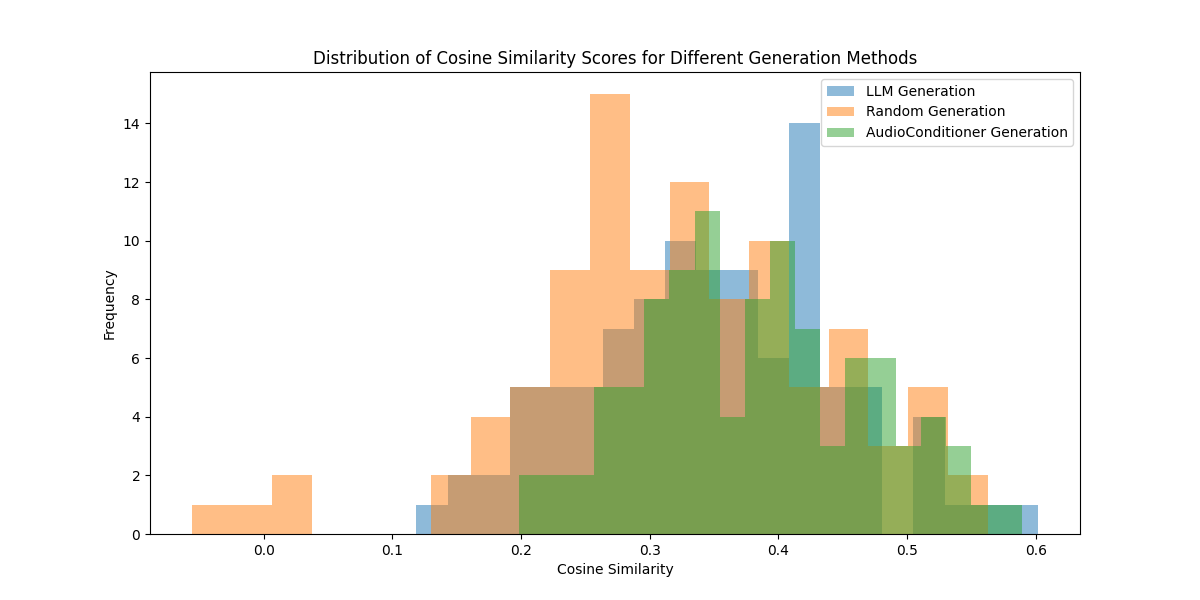
\includegraphics[width=0.7\linewidth]{score_distributions.png}
            \captionof{figure}{CLAP Similarity Distribution (via \texttt{benchmark.py})}
        \end{center}
        \medskip
        \begin{center}
        \begin{tabular}{lc}
        \hline
        Method & Mean CLAP Similarity \\
        \hline
        AudioConditioner & 0.38 \\
        LLM Baseline (Qwen2.5-7B) & 0.35 \\
        Random Baseline & 0.15 \\
        \hline
        \end{tabular}
        \end{center}
        \medskip
        We benchmarked semantic alignment using CLAP cosine similarity between input text and generated audio across 100 held-out samples. AudioConditioner achieved a mean similarity of 0.38, compared to 0.35 for the direct LLM baseline.
}

\column{0.5}

\block{\textsc{Application III: Video Generation \& Orchestration}}{
    We developed the \texttt{video\_sound.py} application to create animated cinematic clips with a synchronized musical score from a single still image.
    \medskip
    
    \textbf{Parallel Execution Pathway:}
    \begin{enumerate}
        \item \textbf{Image Animation:} We parse the input image through the \textbf{CogVideoX} model. As we strictly utilized an open-weight model, the resulting video quality remains limited but serves as a proof-of-concept for the pipeline.
        \item \textbf{Image Orchestration:} Simultaneously, we pass the image directly into the \textbf{AudioConditioner} model to extract visual semantics and produce a matching audio waveform.
        \item \textbf{Multimodal Merging:} We integrate \textbf{FFmpeg} to compile the generated silent video and the generated audio, multiplexing them into a final synced file.
    \end{enumerate}
    \medskip
    
    \begin{center}
    \begin{tikzpicture}[
        node distance=2cm,
        box/.style={rectangle, draw=black, thick, fill=blue!10, text width=6cm, align=center, rounded corners, minimum height=1.5cm},
        imgbox/.style={rectangle, draw=black, thick, fill=gray!20, minimum width=4cm, minimum height=3cm, align=center, font=\itshape},
        arrow/.style={->, thick, >=stealth}
    ]
        
        \node[box, fill=green!10] (img) {\textbf{Source Image}};
        
        \node[box, fill=teal!10] (vid) [below left=2cm and 1cm of img] {CogVideoX};
        \node[box, fill=orange!10] (aud) [below right=2cm and 1cm of img] {Audio Conditioner};
        
        \node[box] (vf) [below=1.5cm of vid] {Silent output.mp4};
        \node[box] (af) [below=1.5cm of aud] {Sound output.wav};
        
        \node[box, fill=red!10] (ffmpeg) [below=9cm of img] {FFmpeg \\ Multiplexing};
        
        \node[box, fill=green!10] (final) [below=1.5cm of ffmpeg] {Final Synced Video};
        
        \draw[arrow] (img.south) -- ++(0,-0.8) -| (vid.north);
        \draw[arrow] (img.south)  -- ++(0,-0.8) -| (aud.north);
        \draw[arrow] (vid) -- (vf);
        \draw[arrow] (aud) -- (af);
        \draw[arrow] (vf.south) |- (ffmpeg.west);
        \draw[arrow] (af.south) |- (ffmpeg.east);
        \draw[arrow] (ffmpeg) -- (final);
        
    \end{tikzpicture}
    \end{center}
    \medskip
    
    These applications demonstrate flexibility across three pipelines for automated scoring, procedural art generation, and multimodal storytelling. We note that the quality of the generated video is lower than the audio quality, with visible artifacts.
}

\block{\textsc{Conclusion \& Future Perspectives}}{
    We demonstrate that \textbf{AudioConditioner} steers music diffusion via a lightweight descriptor bridge trained by knowledge distillation. 
    We achieved three working pipelines — image-to-music, text-to-narrated-audiobook, and image-to-video-with-score — with measurable semantic alignment. 
    \medskip
    
    Future work focuses on contrastive fine-tuning using \textbf{Reinforcement Learning}. By utilizing \textbf{Proximal Policy Optimization (PPO)} with the CLAP similarity score as a dense reward signal, we aim to optimize the descriptor weights to maximize semantic alignment directly. Given that a single audio generation step requires approximately 1 minute, a full PPO training cycle would require several days of continuous execution; however, this would allow the model to discover musical nuances that distillation from a teacher LLM alone may not capture. Longer-term trajectories include human perceptual evaluation and expanded training datasets to further refine the descriptor's precision.
}

\block{\textsc{References}}{
    \begin{itemize}
        \item Li et al. (2022). \textit{BLIP}: Bootstrapping Language-Image Pre-training for Digital Content Understanding.
        \item Elizalde et al. (2023). \textit{CLAP}: Learning Audio Concepts From Natural Language Supervision.
        \item Evans et al. (2024). \textit{Stable Audio Open}: Latent Diffusion for Music Generation.
        \item Chen et al. (2024). \textit{F5-TTS}: A Fully Non-Autoregressive Transformer for TTS.
        \item Yang et al. (2024). \textit{CogVideoX}: Text-to-Video Diffusion with Transformers.
    \end{itemize}
}

\end{columns}
\end{document}
